\documentclass[10pt]{article}


\title{Prediction of Click-through Rates for Ads}

\author{ Abhishek Vijayan     B110158CS\\  Aswathy Ajith     B110759CS\\  Potturi JayaVenkata Sravani    B110903CS\\  Guided by: Dr. Gopakumar G}

\usepackage{epsfig}
\usepackage{graphicx}
\usepackage[margin=0.5in]{geometry}

\graphicspath{ {images/} }
\begin{document}
	
\maketitle
	

\abstract{} 
The online advertising industry is thriving on the learning problem of predicting click through rates for ads. We attempt to propose efficient machine learning techniques that could be used for predicting click through rates with a high degree of accuracy.
\section{Problem Definition}
As part of an online machine learning competition held by KDD Cup, Tencent Corporation released a large data set obtained from the user logs of the search engine soso. The task is to predict the CTR (pCTR) of ads as accurately as possible.
\section{Introduction}
Click-through rate is a very useful metric for ranking and pricing ads in the internet marketing world. It is one of the greatest applications of machine learning. Sponsored search advertising, contextual advertising, display advertising, and real-time bidding auctions have all relied heavily on the ability of learned models to predict ad click–through rates accurately, quickly, and reliably.  A typical industrial model may provide predictions on billions of events per day, using a correspondingly large feature space, and then learn from the resulting mass of data. When a user does a search q, an initial set of candidate ads is matched to the query q based on advertiser-chosen keywords. An auction mechanism then determines whether these ads are shown to the user, what order they are shown in, and what prices the advertisers pay if their ad is clicked. In addition to the advertiser bids, an important input to the auction is, for each ad a, an estimate of P(click | q, a), the probability that the ad will be clicked if it is shown.
\subsection{Literature Survey}
The evaluation metric used in this contest was AUC(Area Under the ROC Curve). AUC gives the probability that a classifier will rank a randomly chosen positive instance higher than a randomly chosen negative one. We will be using the same metric in our project.\\
The Area Under the ROC Curve is found to obtain a single scalar value from the ROC. The value ranges from 0 to 1 with AUC equal to 1 being a perfect classifier. A value of 0.5 indicates a random classifier.\\
AUC is favourable for the following reasons :
\begin{itemize}
	\item No need to choose threshold, favourable when output is not a probability
	\item ROC - insensitive to changes in class-distribution
	\item For skewed class, a classifier that always outputs 0 or 1, will achieve high accuracy. But AUC value will be 0.5 
\end{itemize}
We had done a literature survey on the papers published by the first four winners of KDD Cup 2012.\\
\begin{enumerate}
	\item A Two-Stage Ensemble of Diverse Models for Advertisement Ranking
This approach achieves 0.8069 AUC on the public test set and 0.8089 AUC on the private test set.\\
According to their method, the system can be divided into three stages. They are generating individual models (Different models like Classification models, Regression models, Ranking models, Combined Regression and Ranking models, Matrix Factorization models were used to capture different concepts), blending with the validation set (For increasing the performance, different predictors that were used in first stage were combined) and ensemble learning with the test set (Using Ensemble methods, the blending models are further combined to improve the test set performance)
	\item Ensemble of Collaborative Filtering and Feature Engineered Models for Click Through Rate Prediction
This is a paper by the team Opera Solutions, who stood second on the leaderboard. Their technique had an AUC Score of 0.80824 on the private leaderboard. The methods adopted include Collaborative Filters, Probability Models, Feature Engineered Models. For directly optimizing the AUC, Collaborative Filters and ANN Models were used. Finally these models were blended using an AUC optimized ANN.\\
	\item Click through rate Prediction for Sponsored Search Advertising with Hybrid Models
This solution had secured the 3rd place in KDD cup 2012 track 2. An ensembling is done on a couple of individual methods which include Online Bayesian Probit Regression, Latent Factor Model, Support Vector Machine and Maximum Likelihood Estimation. \\	
	\item A Feature Engineering Approach for Click-Through Rate Prediction
The three main algorithms used were:
Vowpal Wabbit:  Used mainly for Bag of words related models, Linear Mixed Effects(LME) : Used for Statistical features creation, Generalized Boosted Models (GBM) : Used for Model training\\
 
\end{enumerate}
 
\section{Work Done}

\subsection{Data Set}
The types of data provided include training data, additional data and testing data. There are 149,639,105 training instances and 20,297,594 testing instances.\\
Each instance contains at least the following information:\\
UserID, AdID, Query, Depth [number of ads impressed in a session], Position [order of an ad in the impression list], Impression [number of search sessions in which the ad(AdID) was impressed by the user (UserID) who issued the query (Query)], Click [number of times, among the above impressions, the user (UserID) clicked the ad (AdID)]
Fields in the training instance:\\
Click, Impression, DisplayURL [The URL is hashed for anonymity], AdID, AdvertiserID, Depth, Position, QueryID [It is the key of the data file queryid\_tokensid.txt], KeywordID, TitleID [This is the key of titleid\_tokensid.txt], DescriptionID [This is the key of descriptionid\_tokensid.txt], UserID [This is the key of userid\_profile.txt]\\
Besides the details given above, some further details are also provided with additional data files and there are five such files queryid\_tokensid.txt, purchasedkeywordid\_tokensid.txt, titleid\_tokensid.txt, descriptionid\_tokensid.txt, userid\_profile.txt [composed of UserID, Gender, and Age, delimited by the TAB character. Not every UserID in the training and the testing set will be present in 'userid\_profile.txt'. ]
These data files include information such as gender, age ('1'  for (0, 12],  '2' for (12, 18], '3' for (18, 24], '4'  for  (24, 30], '5' for (30,  40], and '6' for greater than 40.)\\
Along with the training data and additional data, the test set is also given which has the same format as the training dataset , except for the counts of ad impressions and ad clicks that are needed for computing the empirical CTR.
\\\\

In the previous semester, we had implemented some basic algorithms on a practice dataset to get a hands on experience in machine learning using octave. Apart from that a literature survey was done so as to get a basic idea of the CTR problem and the generally used methods to solve them. \\\\

One of the major difficulties that we had to encounter while proceeding was to understand the dataset thoroughly and how it could be used. We were expected to predict the CTR value i.e. clicks/impressions. This could be easily modeled as a regression problem by training the model to use the continuous valued CTR as target. To model this as a classification problem, we had to unroll and expand the data. Each tuple is expanded as the number of impressions in the original file. The number of clicks in the original file determine the number of tuples which will carry a 1 in the clicks field. The others will be 0. Thus the impression field is not present in the resulting data set. As we have converted it to a classification problem, the model will now predict the probability with which the ad will be clicked by a particular user which is effectively the CTR. \\\\

We planned to work on a smaller subset of the data for the time being as the original data set is too huge to handle at this point. Randomly, 1000000 tuples were chosen to work with. From that, 60\% was used for training, 20\% for validation and the remaining for testing.\\\\

As per the competition, AUC is used to evaluate the results rather than accuracy. We encountered a problem with the code that was provided as the columns were being wrongly read and hence gave incorrect results. On correcting the code for computing the AUC we were able to make some progress. \\\\

The following graphs depicts how CTR varies with each individual feature.\\

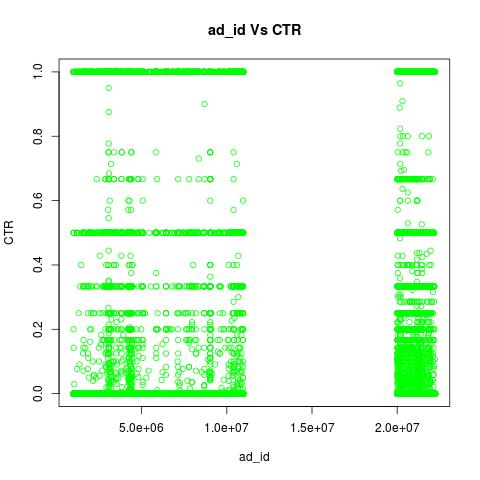
\includegraphics[scale=0.5]{ad_id_Vs_CTR}
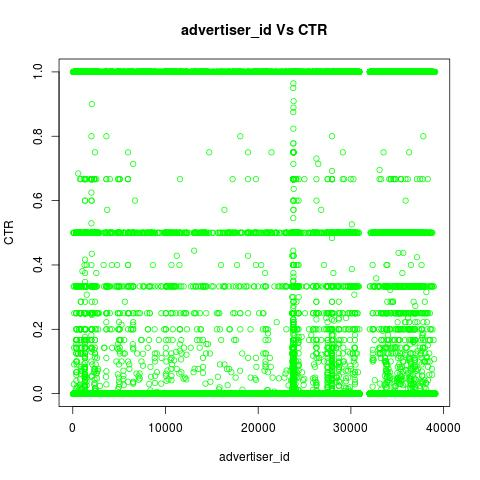
\includegraphics[scale=0.5]{advertiser_id_Vs_CTR}\\\\
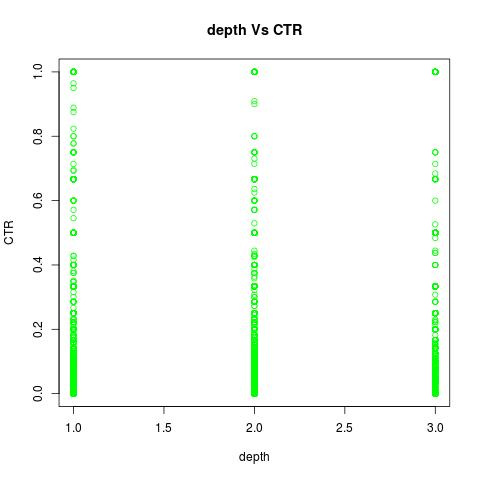
\includegraphics[scale=0.5]{depth_Vs_CTR}
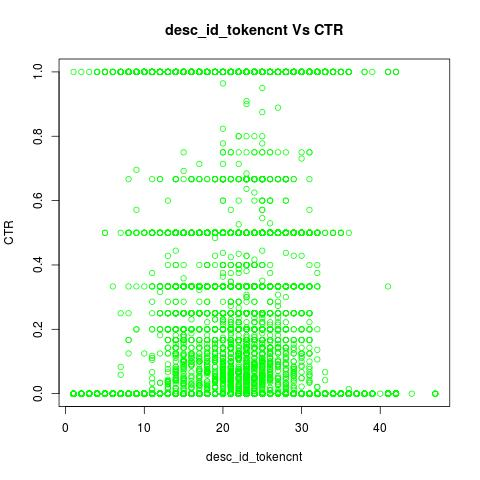
\includegraphics[scale=0.5]{desc_id_tokencnt_Vs_CTR}\\\\
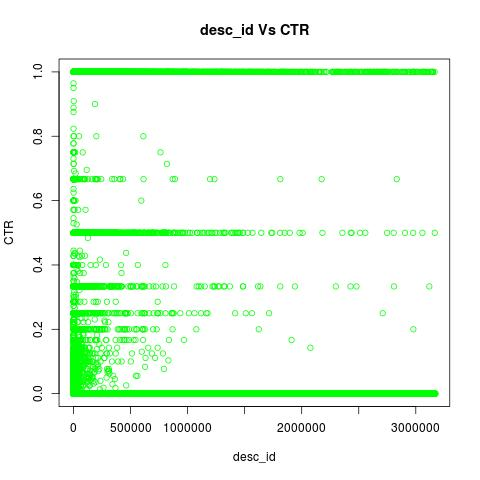
\includegraphics[scale=0.5]{desc_id_Vs_CTR}
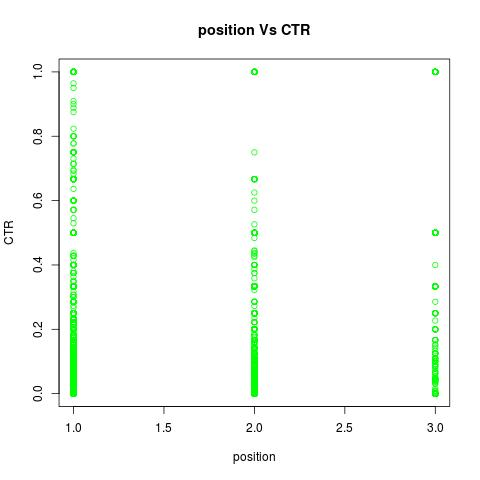
\includegraphics[scale=0.5]{position_Vs_CTR}\\\\
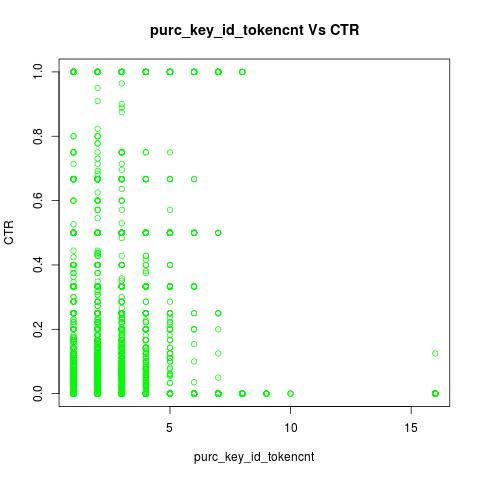
\includegraphics[scale=0.5]{purc_key_id_tokencnt_Vs_CTR}
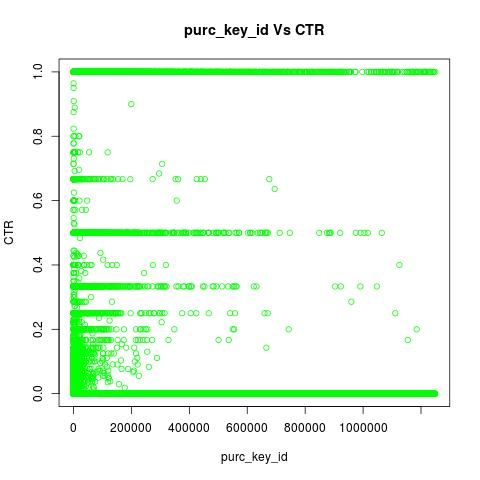
\includegraphics[scale=0.5]{purc_key_id_Vs_CTR}\\\\
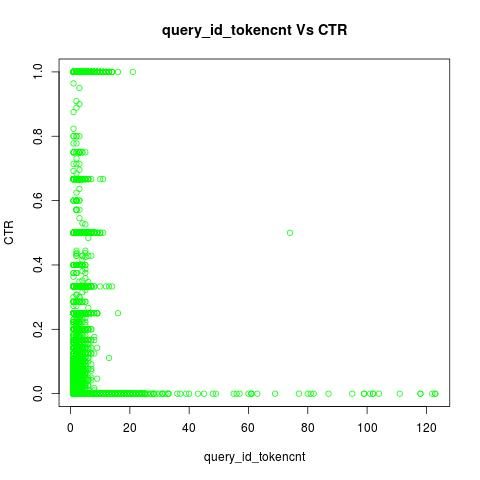
\includegraphics[scale=0.5]{query_id_tokencnt_Vs_CTR}
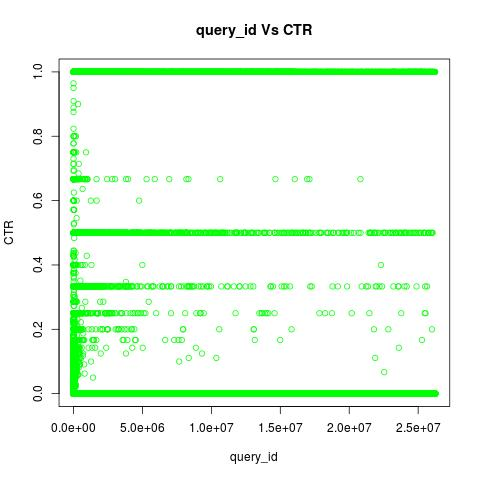
\includegraphics[scale=0.5]{query_id_Vs_CTR}\\\\
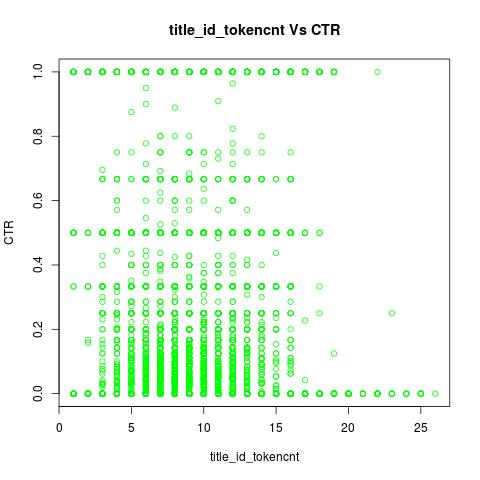
\includegraphics[scale=0.5]{title_id_tokencnt_Vs_CTR}
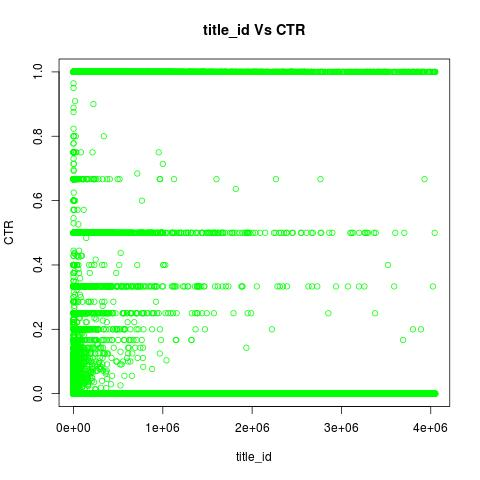
\includegraphics[scale=0.5]{title_id_Vs_CTR}\\\\
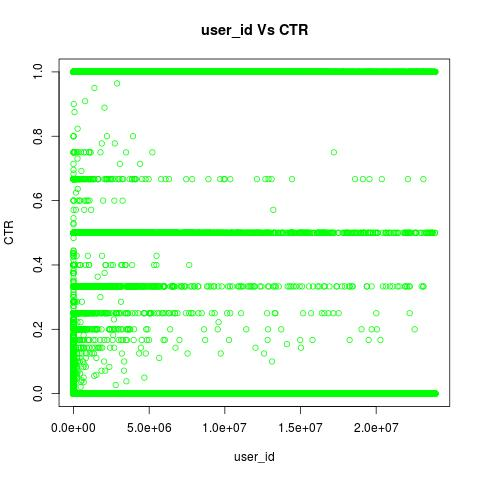
\includegraphics[scale=0.5]{user_id_Vs_CTR}

From these graphs we can infer that there is no direct relationship between any of the indiviual features and the CTR. However, ads with lower position are likely to have a higher CTR.
The additional files that were given needed to be joined with the main data so that better models could be obtained. \\\\

We started working on different tools (Python, R, Vowpal Wabbit) that were new to us. This was necessary as some tools have an edge over the others because of more efficient library implementations while others seem to be faster. \\\\
All our code have been hosted in github : https://github.com/MajorProject-pCTR/Basic \\\\
R \\
R is the most widely used statistical language in data-science competetions. There are efficient inbuilt functions for machine learning algorithms in R. Its disadvantage is that objects must generally be stored in physical memory. \\\\
Octave \\
Octave is the open-source variant of Matlab. Its efficient vectorized computations have been used in our implementations. The performance of this language is also limited by primary memory.\\\\

Python\\
The tasks were implemented using scikit-learn and numpy. Scikit-learn is used for classification, feature selection, feature extraction and clustering.\\\\

Vowpal Wabbit\\
Vowpal Wabbit is an open source machine learning library developed by Yahoo. It is implemented using Online Machine Learning techniques. Vowpal Wabbit is out-of-core i.e., designed to even handle the data that cannot be fit in the primary memory by accessing data from hard drives.\\\\

Here are the results that we obtained.

\section{Results}
\subsection{Linear regression}
\subsubsection{Python}
\begin{center}
 \begin{tabular}{|c | c | c | c||} 
 \hline
 & Training AUC & Testing AUC & Total time\\ [0.5ex] 
 \hline\hline
Before join & 0.586956 & 0.604606 & 34.114s\\
 \hline
After join & 0.586956 & 0.604606 & 28.680s\\ 
 \hline
\end{tabular}
\end{center}

\subsubsection{Vowpal Wabbit}

Linear Regression:\\

\begin{center}
 \begin{tabular}{|c | c | c||} 
 \hline
 & Training & Testing\\ [0.5ex] 
 \hline\hline
AUC & 0.589910 & 0.626719\\ 
 \hline
Time & 21.828s & 7.759s\\ 
 \hline
\end{tabular}
\end{center}

Linear Regression with quantile loss function:\\

\begin{center}
 \begin{tabular}{|c | c | c||} 
 \hline
 & Training & Testing\\ [0.5ex] 
 \hline\hline
AUC & 0.511265 & 0.511187\\ 
 \hline
Time & 20.827s & 7.257s\\ 
 \hline
\end{tabular}
\end{center}

\subsubsection{R}

\subsection{Logistic regression}
\subsubsection{Python}

\begin{center}
 \begin{tabular}{|c | c | c | c||} 
 \hline
 & Training AUC & Testing AUC & Total time\\ [0.5ex]
 \hline\hline
Before join & 0.507160 & 0.474355 & 34.114s\\
 \hline
After join & 0.507160 & 0.474355 & 34.114s\\ 
 \hline
\end{tabular}
\end{center}

\subsubsection{R}

\subsection{Neural networks}
\subsubsection{Vowpal Wabbit}
Before joining the main data set with the additional files, Neural Network gave best results with 8 nodes in the hidden layer:\\

\begin{center}
 \begin{tabular}{|c | c | c | c||} 
 \hline
 & Training & Validation & Testing\\ [0.5ex] 
 \hline\hline
AUC & 0.514684 & 0.632026 & 0.647415\\
 \hline
Time & 29.861s & 8.509s & 17.910s\\ 
 \hline
\end{tabular}
\end{center}

After joining the main data set with the additional files, Neural Network gave best results with 5 nodes in the hidden layer:\\

\begin{center}
 \begin{tabular}{|c | c | c | c||} 
 \hline
 & Training & Validation & Testing\\ [0.5ex] 
 \hline\hline
AUC & 0.637832 & 0.604052 & 0.602947\\
 \hline
Time & 11.455s & 9.341s & 8.078s\\ 
 \hline
\end{tabular}
\end{center}
\subsubsection{R}

\subsection{Random forests}

\begin{center}
 \begin{tabular}{|c | c | c | c||} 
 \hline
 & Training AUC & Testing AUC & Time\\ [0.5ex] 
 \hline\hline
Before join & 0.981369 & 0.620459 & 2m20.759s\\
 \hline
After join & 0.979796 & 0.608228 & 2m20.759s\\ 
 \hline
\end{tabular}
\end{center}

\subsection{Ensemble}
We have tried ensembling the individual results using neural nets. Ensemble of Linear Regression and Neural Network with 8 nodes in hidden layer(Using Linear Regression) gives the following result:\\

\begin{center}
 \begin{tabular}{|c | c | c||} 
 \hline
 & Training & Testing\\ [0.5ex] 
 \hline\hline
AUC & 0.556894 & 0.533243\\ 
 \hline
Time & 28.621s & 10.838s\\ 
 \hline
\end{tabular}
\end{center}

\section{Proposed Method}
We propose to improve the newly found AUC by different means by varying the parameter values, deriving new features by combining existing features and trying out alternate combinations of basic algorithms for blending.
\section{Future Work}
Some more complex algorithms namely SVM and Collaborative Filtering will be next tried on this data subset. Efficient methods for ensembling using Neural Networks and random forest will be done. The complete dataset will be used with Vowpal Wabbit as the tool. If Vowpal Wabbit isn't efficient enough, then a cluster will be set up and the machine learning algorithms already used and others on the paper will be implemented on it. With this, hopefully we would be able to improve the AUC obtained in the paper or otherwise get an approximately same AUC.
\section{Conclusion}
We managed to get a good grip over the data and obtained a sufficiently small subset of it for local implementation. Some machine learning techniques including linear regression, logistic regression, neural nets and random forests were implemented in the smaller data set using different machine learning tools such as Python, Vowpal Wabbit and R, we are working on getting the subset of the original data set of our problem that represents the original data set so that first we can work on that subset in our local machine.
\section{Bibliography}
\begin{enumerate}
	\item KDD Cup 2012, https://www.kddcup2012.org/c/kddcup2012-track2
	\item Machine Learning by Andrew Ng, https://class.coursera.org/ml-006
	\item An Introduction to Statistical Learning with Applications in R : By Gareth James, Daniela Witten, Trevor Hastie and Robert Tibshirani
	\item An Introduction to R : By W. N. Venables, D. M. Smith and the R Core Team
	\item scikit-learn Machine Learning in Pythonhttp://scikit-learn.org/stable/
	\item Convex Optimized - Vowpal Wabbit tutorial for the Uninitiated http://zinkov.com/posts/2013-08-13-vowpal-tutorial/
	\item JohnLangford/vowpal\_wabbit https://github.com/JohnLangford/vowpal\_wabbit/wiki
	\item Ensemble of Collaborative Filtering and Feature Engineered Models for Click Through Rate Prediction https://kaggle2.blob.core.windows.net/competitions/kddcup2012/2748/media/Opera.pdf
	\item A Two-Stage Ensemble of Diverse Models for Advertisement Ranking in KDD Cup 2012 https://kaggle2.blob.core.windows.net/competitions/kddcup2012/2748/media/NTU.pdf
	\item Click-Through Prediction for Sponsored Search Advertising with Hybrid Models https://kaggle2.blob.core.windows.net/competitions/kddcup2012/2748/media/CAS.pdf
	\item A Feature Engineering Approach for Click-Through Rate Prediction https://kaggle2.blob.core.windows.net/competitions/kddcup2012/2748/media/BirutasTeam.pdf
\end{enumerate}
\bibliographystyle{unsrt}	

\nocite{*}		

\bibliography{bibname}		


\end{document}
